\documentclass[12pt,a4paper]{report}
\usepackage[ngerman]{babel}
\usepackage{../../vpl}
\graphicspath{{../../images/}}

% localized boxes
\newcommand*{\trickbox}[1]{\infobox{Trick}{#1}{blue!10}{\bclampe}}
\newcommand*{\importantbox}[1]{\infobox{Wichtige Information}{#1}{yellow!10}{\bcinfo}}
\newcommand*{\yourturnbox}[1]{\infobox{Ihre Umdrehung}{#1}{orange!10}{\bccrayon}}
\newcommand*{\exercisebox}[2]{\infobox{Übung #1}{#2}{orange!10}{\bccrayon}}
\newcommand*{\warningbox}[1]{\infobox{Achtung !}{#1}{orange!10}{\bcattention}}

\begin{document}
\thispagestyle{empty}

\begin{center}
\begin{Huge}
\begin{bfseries}
Erste Schritte in der Robotik
\end{bfseries}

mit dem 

\begin{bfseries}
Thymio-II Roboter
\end{bfseries}

und der

\begin{bfseries}
Aseba/VPL Umgebung
\end{bfseries}

\end{Huge}

\vskip 2cm


\begin{LARGE}
\href{http://www.weizmann.ac.il/sci-tea/benari/}{Moti Ben-Ari} und andere Mitwirkende\\
\end{LARGE}
\bigskip
\begin{Large}
Details in \texttt{authors.txt} 
\end{Large}

\vskip 1cm

\begin{Large}
Version 1.1 für \href{https://aseba.wikidot.com/de:downloadinstall}{Aseba 1.3.1}
\end{Large}

\end{center}

\vfill

\begin{center}
\copyright{}\  2013 \href{http://www.weizmann.ac.il/sci-tea/benari/}{Moti Ben-Ari} und andere Mitwirkende.
\end{center}

Dieser Inhalt ist unter der Creative-Commons-Lizenz vom Typ Namensnennung -
Weitergabe unter gleichen Bedingungen 3.0 Unported lizenziert.
Um eine Kopie dieser Lizenz einzusehen, besuchen Sie \url{http://creativecommons.org/licenses/by-sa/3.0/} oder schreiben Sie einen Brief an Creative Commons, 444 Castro Street, Suite 900, Mountain View, California, 94041, USA.

\begin{center}
\includegraphics[width=.2\textwidth]{../images/by-sa}
\end{center}

\tableofcontents
\thispagestyle{empty}
\chapter*{Vorwort}
\sect{Was ist ein Roboter?}
Sie fahren mit ihrem Fahrrad und plötzlich sehen sie, dass die Strasse vor ihnen aufwärts geht. Sie treten kräftiger in die Pedale, um den Rädern mehr Energie zuzuführen. Dadurch werden sie auch aufwärts nicht langsamer. Nachdem sie oben angekommen sind, geht es wieder runter. Sie betätigen die Bremsen ihres Fahrrads wodurch sie nicht zu schnell werden. Wenn sie Fahrrad fahren, sind ihre Augen wie \textit{Sensoren}, die ihre Umgebung wahrnehmen. Wenn diese Sensoren — ihre Augen — ein \textit{Ereignis} erfassen (zum Beispiel eine Kurve), führen sie eine \textit{Aktion} aus (zum Beispiel den Fahrradlenker nach links oder rechts zu bewegen).

In einem Auto sind Sensoren eingebaut, die \textit{messen} was in der Umgebung passiert. Der Tachometer misst, wie schnell das Auto fährt. Wenn sie sehen, dass das Auto schneller als das Tempolimit fährt, sagen sie dem Fahrer, er fahre zu schnell. Darauf kann der Fahrer eine Aktion ausführen, nämlich die Bremse betätigen, damit das Auto langsamer wird. Die Tankanzeige misst, wie viel Benzin noch im Tank des Autos ist. Wenn sie sehen, dass die Anzeige zu tief ist, können sie der Fahrerin sagen, dass sie eine Tankstelle suchen muss. Sie kann dann eine Aktion ausführen: Sie kann den Blinker einschalten und das Steuerrad nach rechts drehen, um zur Tankstelle zu fahren.

Jeder Fahrradfahrer und Autofahrer erhält Informationen von den Sensoren, entscheidet dann welche Aktion nötig ist und führt diese Aktionen aus. Ein \textit{Roboter} ist ein System, in welchem dieser Prozess — Informationen erhalten, Entscheidungen treffen, Aktionen ausführen — von einem Computer durchgeführt wird. Normalerweise macht der Roboter das ohne die Hilfe von Menschen.

\sect{Thymio Roboter und Aseba VPL Umgebung}
Thymio ist ein kleiner Roboter, der für pädagogische Zwecke entwickelt wurde (\cref{fig.front}). Die Sensoren des Roboters messen Licht, Töne und Distanzen und detektieren, ob Knöpfe gedrückt werden oder ob an den Roboter geklopft wird. Die wichtigste Aktionen, die durchgeführt werden kann, ist die Bewegung durch zwei Räder, die mit je einem Motor angetrieben werden. Weitere Aktionen sind das Erklingen lassen von Tönen und das Ein- und Ausschalten von Lichtern in verschiedenen Farben.

In diesem Dokument sprechen wir jeweils von Thymio, obwohl natürlich die aktuelle Version Thymio II gemeint ist. 

Aseba ist eine Programmierumgebung für kleine Roboter, wie Thymio. VPL ist ein Teil von Aseba und dient der visuellen Programmierung (visual programming). VPL wurde entwickelt, um Thymio auf einfache Art und Weise mit Ereignis- und Aktionsblöcken programmieren zu können.

%\newpage
\sect{Tutorialübersicht}

Jedes Kapitel befasst sich mit einem besonderen Thema, welches aus der kurzen Einleitung hervor geht, gefolgt von der Darstellung der Ereignisse und Aktionsblöcke, die jeweils verwendet werden. Es wird empfohlen, zunächst die Kapitel im Standard-Modus zu bearbeiten, später den Fortgeschrittenen-Modus zu untersuchen oder einige Projekte zu versuchen. Das Parson-Rätsel soll versuchen, wer sein Wissen über VPL testen will. Lesen Sie \cref{ch.next} sobald Sie VPL verlassen möchten, um sich der erweiterten Umgebung von Aseba Studio zu widmen. Die Anhänge umfassen Referenzmaterialien, die bei Bedarf gelesen werden sollen. 

\subsection*{Teil I: Tutorial}

\textbf{\cref{ch.intro,ch.colors}} geben eine grundlegende Einführung in den Roboter, die VPL-Umgebung und ihr wichtigstes Programmierkonstrukt: das Ereignis-Aktionen-Paar.

\textbf{Ereignis}: Tasten \hfill \textbf{Aktionsblöcke}: Farbe der oberen und unteren Lichter

\blkmed{event-buttons} \hfill \blkmed{action-colors-up} \quad \blkmed{action-colors-down}

\medskip

\textbf{\cref{ch.moving,ch.pet,ch.line}} erklären die Aktionen und Algorithmen für autonome mobile Roboter. Sie stellen sicher den Kern jeder Beschäftigung mit Thymio und VPL dar. 

\textbf{Ereignis}: Tasten, Distanzsensoren \hfill
\textbf{Aktionsblöcke}: Motoren

\blkmed{event-buttons} \quad\blkmed{event-prox}\quad \blkmed{event-prox-ground} \hfill
\blkmed{action-motors}

\medskip

\textbf{\cref{ch.bells}} beschreibt Funktionen des Roboters, deren Verwendung Spass macht, die aber nicht wesentlich sind: Geräusche und Erschütterungen.

\textbf{Ereignis}: Berührung, Klatschen \hfill \textbf{Aktionsblöcke}: Melodie, Farbe der Lichter

\blkmed{event-tap} \quad \blkmed{event-clap} \hfill \blkmed{action-music}
\quad \blkmed{action-colors-up} \quad \blkmed{action-colors-down}

\medskip

\importantbox[Fortgeschrittener Modus]{VPL hat einen Standard-Modus, der elementare Ereignisse und Aktionen unterstützt, die für Anfänger einfach zu meistern sind. Der erweiterte Modus von VPL unterstützt weitere Ereignisse und Aktionen, die einen Anfänger überfordern würden, aber für den Fortgeschrittenen hilfreich sind. Er beginnt ab \cref{ch.time}.}

\medskip

\textbf{\cref{ch.time}} erklärt zeit-bezogene Ereignisse. Es gibt einen Aktionsblock um einen Timer (Wecker) zu stellen; sobald der Timer abgelaufen ist, tritt das Ereignis ein. 

\textbf{Ereignis}: Zeit abgelaufen \hfill \textbf{Aktionsblöcke}: Timer setzen

\blkmed{event-timer} \hfill \blkmed{action-timer}

\newpage

\textbf{\cref{ch.states,ch.counting}} erklären Zustands-Maschinen, welche es dem Roboter erlauben, bestimmte Aktionen zu unterschiedlichen Zeitpunkten durchzuführen. Zustände können auch verwendet werden, um elementare arithmetische Operationen auszuführen wie das Zählen.

\textbf{Ereignis}: Zustand (bezogen auf Ereignis) \hfill \textbf{Aktionsblöcke}:
ändern des Zustands

\blkmed{state-filter} \hfill \blkmed{action-states}

\medskip

\textbf{\cref{ch.angles}} beschreibt, wie man die Beschleunigungsmesser von Thymio verwendet.

\textbf{Ereignis}: Beschleunigungsmesser

\blkmed{event-pitch} \quad \blkmed{event-roll}

\bigskip

\subsection*{Teil II: Parson-Rätsel}

\textbf{\cref{ch.parsons}} stellt die Parson-Rätsel vor, mit denen man das Wissen über VPL testen kann.

\bigskip

\subsection*{Teil III: Projekte}

\textbf{\cref{ch.brait,ch.rabbit,ch.barcode,ch.sweep,ch.speed,ch.radar,ch.fa,ch.slow,ch.two}}
spezifizieren Projekte, die man selbständig designen und implementieren kann. Der passende Quellcode findet man im Archiv, es wird aber empfohlen, zunächst eine selbständige Lösung zu erarbeiten!

\bigskip

\subsection*{Teil IV: Übergang von visueller zu textbasierter Programmierung}

\textbf{\cref{ch.next}} verweist auf den nächsten Schritt: die Verwendung der textbasierten Programmierung mit Aseba-Studio. Diese bietet deutlich mehr Funktionen für die Entwicklung von Robotern als VPL.

%\informationbox{Reference material}{The appendices contains reference
%material that you will want to look at from time to time to learn about
%new featuers of VPL or to refresh your memory.}
\bigskip

\subsection*{Teil V: Anhänge}

\textbf{\cref{a.toolbar}} enthält eine Beschreibung der Benutzerschnittstelle---die Knöpfe in der Toolbar.
%It also describes how to display dynamic feedback when a VPL program is run.

\textbf{\cref{a.blocks}} zählt die Ereignisse auf und die Aktionsblöcke des Standard- und der Fortgeschrittenen-Modus. 

\textbf{\cref{a.tips}} enthält Leitlinien für Lehrer und
Mentoren. Der erste Abschnitt zeigt, wie man das entdeckende Lernen und das Experimentieren fördern kann. Der nächste Abschnitt konzentriert sich auf gutes Programmieren. Der letzte Abschnitt listet einige Probleme auf, auf die man stossen kann und bietet Hinweise, wie diese zu überwinden sind.

\textbf{\cref{a.tech}} beschreibt Techniken im Umgang mit den Schiebereglern der Motoren und Sensoren.

\blkmed{event-prox-advanced} \quad \blkmed{event-prox-ground-advanced}


\sect{Referenzkarten}

Es mag hilfreich sein, eine oder beide VPL-Referenzkarte(n) auszudrucken. Sie sind in dem Zip-File enthalten, woher Sie diese Beschreibung haben; sie sind aber auch unter folgendem Link verfügbar: \href{https://www.thymio.org/de:visualprogramming}{https://www.thymio.org/de:visualprogramming}.

\begin{itemize}
\item Übersicht über die Ereignis und Aktions-Blöcke auf einer Seite.
\item Ein zweiseitiges Dokument, das zu einer handlichen Karte gefaltet werden kann. Sie fasst die Benutzeroberfläche, die Ereignis- und Aktions-Blöcke zusammen und enthält einige Beispiele.
\end{itemize}

\sect{Aseba installieren}

Um Aseba zu installieren (inkl. VPL), gehen sie auf folgende Seite 
\href{https://www.thymio.org/de:start}{https://www.thymio.org/de:start}
und klicken sie auf das Icon mit ihrem Betriebssystem (Windows, Mac OS, etc.). Folgen sie der Anleitung zum Download und zur Installation der Software. Die Aseba-Installation umfasst neben der VPL auch die Entwickler-Umgebung Aseba Studio (siehe \cref{ch.next}).

\part{Tutorial}

\chap{Ihr erstes Roboter-Projekt}\label{ch.intro}

\sect{Thymio kennen lernen}

\Cref{fig.front} zeigt den Roboter Thymio von vorne und von oben. Oben sieht man einen runden Knopf in der Mitte (\textcolor{blue}{A}) und die vier Richtungsknöpfe (\textcolor{blue}{B}). Hinter den Knöpfen wird der Ladezustand der Batterie in grün (\textcolor{blue}{C}) angezeigt. Dahinter sieht man die zwei oberen Lichter (\textcolor{blue}{D}), die auf rot eingestellt sind. Der Roboter hat unten weitere solche Lichter (siehe \Cref{fig.bottom}). Die schmalen schwarzen Rechtecke (\textcolor{blue}{E}) vorne sind Sensoren, die Sie im \cref{ch.pet} kennenlernen werden. 

\begin{figure}[h]
\begin{center}
\gr{front}{.8}
\caption{Thymio Roboter von vorne oben}\label{fig.front}
\end{center}
\end{figure}

\sect{Den Roboter verbinden und VPL starten}

Verbinden Sie Ihren Thymio Roboter mit dem USB Kabel mit dem Computer. Der
Roboter spielt eine kleine Tonabfolge ab und die Oberfläche leuchtet grün. Sollte der Roboter ausgeschaltet sein oder bei der Verbindung sich nicht einschalten, schalten sie ihn ein, indem sie während fünf Sekunden
den mittleren Knopf berühren. Starten sie nun VPL indem sie das VPL-Icon \blksm{thymiovpl} auf ihrem Computer mit Doppelklick anwählen.

\importantbox[Kleine Bilder]{Wenn ein kleines Bild im Text erscheint, wird eine grosse Version davon am Rand dargestellt.}

Möglicherweise verbindet sich VPL automatisch mit ihrem Roboter. Falls dies nicht der Fall sein sollte, wird das Bild wie in \cref{fig.connect} angezeigt. Wählen Sie das Kästchen \bu{Serie} an, klicken Sie auf \bu{Thymio-II Robot ...} darunter, wählen sie die Sprache und klicken sie auf \bu{Verbinden}. Abhängig von der Konfiguration ihres Computers und des Betriebssystems, das sie einsetzen, kann es sein, dass die Einträge im Fenster und die folgenden Daten des Thymio etwas anders ausschauen, als in der Abbildung angezeigt.

\trickbox{Es ist auch möglich VPL aus dem Aseba Studio (textbasierte Programmierumgebung) heraus zu öffnen. Das VPL Plug-in befindet sich unten links im Fenster unter \textit{Tool}.} 

\begin{figure} 
\begin{center}
\gr{connect}{.4}
\caption{Thymio mittels USB-Kabel verbinden}\label{fig.connect}
\end{center}
\end{figure}

\sect{Wireless Thymio}

Es gibt eine Thymio-Version, die der Fähigkeit zur drahtlosen Kommunikation besitzt. Diese müssen nicht via Kabel verbunden werden. Der Wireless-Roboter wird mit einem kleinen Objekt ausgeliefert, dem sogenannten \emph{Dongle}:

\gr{dongle}{.4}

Stecken Sie den Dongle in einen USB-Steckplatz Ihres Computers, schalten Sie den Roboter ein und starten Sie VPL, wie weiter oben beschrieben. Wenn Sie das Verbindungsfenster sehen (Abbildung \ref{fig.connect}) wählen Sie die Zeile mit der Bezeichnung \bu{Thymio-II Wireless (COMnn)}.

\importantbox{Sie benötigen immer noch ein USB-Kabel um den Roboter aufzuladen (Abbildung~\ref{fig.back}).}

\sect{Bedienungsoberfläche von VPL}

Die Bedienungsoberfläche von VPL wird unten angezeigt. Diese ist in sechs
Bereiche aufgeteilt:
\begin{enumerate}[noitemsep,nosep]
\item Oben hat sie eine Symbolleiste mit Symbolen, um Programme zu öffnen, zu speichern, auszuführen, etc.
\item Unterhalb der Symbolleiste befindet sich der Bereich, in dem man Programme für den Roboter erstellt.
\item  In einem Nachrichten-Bereich wird angezeigt, ob das Programm funktioniert oder es werden Fehlermeldungen angezeigt.
\item Links eine Spalte mit den Ereignisblöcken.
\item Weiter rechts eine Spalte mit den Aktionsblöcken zur Konstruktion des Programms.
\item Auf der rechten Seite der Code, wie das Programm in die textbasierte Sprache von Aseba übersetzt wird.
\end{enumerate}

\plainfloat
\begin{figure}[h]
\gr{gui}{1}
\caption{Die Bedienungsoberfläche von VPL}\label{fig.vplgui}
\end{figure}
\framedfloat

\newpage

\informationbox{Weiterführende Informationen}{ Wenn Sie mit VPL ein Programm erstellen, wird eine Übersetzung in die textbasierte Programmiersprache AESL vorgenommen. Diese erscheint im Fenster rechts (Bereich 6. in der Abbildung). Dabei handelt es sich um das AESL Programm, welches gerade auf dem Roboter ausgeführt wird. Falls Sie mehr über AESL wissen wollen, werden Sie beim \cref{ch.next} fündig, wo diese Übersetzung erklärt wird.
Weitere Informationen finden Sie unter 
\href{https://www.thymio.org/de:asebausermanual}{https://www.thymio.org/de:asebausermanual} (Lern- und Referenzmaterial zu AESL und Aseba Studio).}



\sect{Ein Programm erstellen}

Beim Start von VPL erscheint ein leerer Programmierbereich.

Falls Sie diesen Programmierbereich zurücksetzen wollen, nachdem Sie programmiert haben und neu beginnen wollen, klicken Sie auf \blksm{new} (\bu{Neu}).

Ein VPL-Programm besteht aus einem Paar oder mehreren Paaren von \emph{Ereignis-
	und Aktions-Blöcken}. Ein Beispiel; das Paar: \blkc{e-a-pair} die oberen Lichter werden auf rot gewechselt, wenn der vordere Knopf berührt wird. 

\importantbox[Wichtiger Hinweis]{Die Bedeutung eines Ereignis-Aktions-Paares ist:\\\textbf{\textit{Wenn das Ereignis eintritt, wird die Aktion durchgeführt.}}
}

Der Programmierbereich besteht zu Beginn aus einem leeren Rahmen für ein Ereignis-Aktions-Paar: \blkc{empty-frame} Um einen Block in den Programmierbereich zu bringen, wählt man ihn mit der Maus aus (Bereiche 4 und 5 in der \cref{fig.vplgui}), und verschiebt ihn bei gedrückter Maustaste in das gestrichelte Quadrat. Sobald der Block über dem Quadrat ist, lässt man den Mausknopf wieder los und platziert damit den Block entsprechend.

\importantbox[Wichtiger Hinweis]{Die beschriebene Technik nennt man \emph{drag-and-drop} und wird häufig verwendet bei grafischen Benutzeroberflächen.}

Beginnen Sie mit dem Ereignis-Knopf \blksm{event-buttons}, indem Sie diesen von der linken Ereignis-Auswahl in das linke Quadrat ziehen. Wählen Sie nun den Aktionsblock für das obere Licht \blksm{action-colors-up} aus der rechten Auswahl und ziehen Sie ihn in das rechte Quadrat. Sie haben nun Ihr erstes Ereignis-Aktions-Paar erstellt.

Jetzt müssen wir das Ereignis und die Aktion so verändern, dass sie das machen was wir wollen. Beim Ereignis können wir zum Beispiel auf den Vorwärts-Knopf klicken; er wird dann rot: \blkc{forward}

Das bedeutet, dass \textbf{ein Ereignis stattfindet, wenn der Vorwärts-Knopf auf dem Thymio Roboter gedrückt wird}.

Der Farbaktionsblock (Aktions-Block für das Licht) hat drei Balken mit den Grundfarben Rot, Grün und Blau.
Jeder dieser Balken hat ganz links ein weisses Quadrat. Die farbigen Balken mit dem weissen Quadrat werden Schieberegler (slider) genannt. Verschieben Sie das Quadrat von links nach rechts und Sie sehen, wie sich die Hintergrundfarbe des Blocks verändert - die Farbe entspricht der späteren Farbe des Roboters. Alle Farben können durch Mischen der drei Grundfarben Rot, Grün und Blau erstellt werden.
Schieben Sie das Quadrat im roten Balken nun ganz nach rechts und die Quadrate im grünen und blauen Balken ganz nach links. Die Farbe des Roboters
leuchtet nun rot, ohne blau und ohne grün: \blkc{red}

\sect{Speichern des Programms}

Bevor Sie Ihr erstes Programm ausführen können, müssen Sie es speichern. Klicken Sie auf das Symbol \blksm{save} in der Symbolleiste. Sie müssen dem Programm nun einen Namen geben; wählen Sie einen Namen, der Ihnen später hilft, sich daran zu erinnern was das Programm macht (zum Beispiel: \bu{rot leuchten}). Wählen Sie einen Ort, wo Sie das Programm speichern möchten, z.B. auf dem Schreibtisch (Desktop) und drücken Sie \bu{Speichern}.

\importantbox[Regelmässig speichern]{Wenn Sie ein Programm ändern, vergessen Sie nicht, regelmässig zu \bu{Speichern}, um die gemachten Änderungen nicht zu verlieren.}

\sect{Ausführen des Programms}

Um das Programm auszuführen, müssen Sie auf das Symbol \blksm{run} \bu{Laden und ausführen} klicken. Nun können Sie den Vorwärts-Knopf auf den Roboter berühren und dann sollte der Roboter rot leuchten. 

\informationbox{Gratulation!}{Sie haben Ihr erstes Programm erstellt und ausgeführt! Das Verhalten des Programms ist: \\
	\textbf{Wenn der Vorwärtsknopf gedrückt wird, wird der Roboter oben rot.}
}

Falls Sie das VPL Programm stoppen möchten, klicken Sie auf \blksm{stop}, die rote (\bu{Halten})-Taste.
Dies ist wichtig, wenn ein Programm den Roboter bewegt, aber das Ereignis-Aktions-Paar für ein Anhalten nicht hinzugefügt wurde. 

\sect{Den Roboter ausschalten}

Um den Roboter auszuschalten, drücken Sie den mittleren Knopf für fünf Sekunden bis Sie eine Tonfolge hören. Der Akku des Roboters wird weiter aufgeladen, solange das Kabel an einen eingeschalteten Computer angeschlossen ist. Der Akku lädt, wenn das kleine Licht neben dem USB Stecker rot leuchtet. Wenn es blau leuchtet, ist der Akku vollständig aufgeladen (\cref{fig.back}) - der Roboter kann nun vom USB-Kabel getrennt werden.

\trickbox{Der Akku wird schneller aufgeladen, wenn Sie ein Ladegerät eines Smartphones verwenden mit einem Micro-USB-Adapter.}

\begin{figure}
\begin{center}
\gr{back}{.6}
\caption{Die Rückseite von Thymio mit USB-Kabel und LED Ladeanzeige}\label{fig.back}
\end{center}
\end{figure}

Sollte die Verbindung des USB-Kabels während des Programmierens nicht funktionieren, blockiert VPL bis die Verbindung wieder hergestellt wird. Kontrollieren Sie beide Enden des Kabels, stellen Sie die Verbindung wieder her und schauen Sie, ob VPL wieder funktioniert. Falls ein Problem auftaucht, können Sie VPL schliessen, den Roboter neu anschliessen und VPL neu starten.

%\newpage

\sect{Ein Programm ändern}

\begin{itemize}
	\item Um ein Ereignis-Aktions-Paar zu löschen, klicken Sie auf \blksm{x}, das oben rechts neben jedem Paar angezeigt wird.
	\item Um ein weiteres Ereignis-Aktions-Paar hinzuzufügen, klicken Sie auf \blksm{plus}, das in der Mitte unter jedem Paar  angezeigt wird.
	\item Um ein Ereignis-Aktions-Paar zu verschieben, können Sie es einfach an die neue Position ziehen.
	\item Um ein Ereignis-Aktions-Paar an eine andere Stelle im Programm zu kopieren, drücken Sie die Taste \bu{Ctrl} oder \bu{Strg} und ziehen Sie das Paar mit der Maus an die entsprechende Stelle.\label{p.copy-pairs}\footnote{Unter OSX (Mac) wird die Taste \bu{Command} verwendet}
\end{itemize}

\informationbox{Der blinkende \bu{Laden und Ausführen} Knopf}{Wenn Sie ein Programm verändern, beginnt der Knopf \bu{Laden und Ausführen} in grüner und blauer Farbe zu blinken, was Sie daran erinnern soll, dass Sie diesen Knopf betätigen müssen, um das veränderte  Programm auf den Roboter zu laden. \label{p.blink}}

Falls Sie mit einem Programm experimentieren wollen, können Sie das bestehende Programm unter einem neuen Namen speichern, um so das ursprüngliche Programm nicht zu verlieren. Klicken Sie dazu einfach auf \blksm{saveas} (\bu{Speichern unter}) und geben Sie einen entsprechenden Namen ein.

\sect{Ein Programm öffnen}

Angenommen Sie haben Ihr Programm gespeichert und den Roboter ausgeschaltet,
möchten aber später wieder an Ihrem Programm weiter arbeiten. Verbinden Sie dazu den Roboter wie beschrieben und klicken Sie dann auf \blksm{open} \bu{Öffnen} und wählen Sie  das Programm, das Sie öffnen möchten (zum Beispiel \bu{rot-leuchten}). Das Programm wird jetzt im Programmierbereich angezeigt und Sie können es verändern.

\sect{Das aktuelle Ereignis-Aktions-Paar}

Wenn man ein Ereignis-Aktions-Paar anklickt, wird sein Hintergrund gelb. Dies geschieht ebenso, wenn man ein Ereignis oder eine Aktion in einen leeren Block eingibt:

\begin{center}
\begin{tabular}{c@{\hspace{.1\textwidth}}c}
\includegraphics[width=.3\textwidth,keepaspectratio=true]{event-action-pair-yellow1}
&
\includegraphics[width=.3\textwidth,keepaspectratio=true]{event-action-pair-yellow2}
\end{tabular}
\end{center}

Das linke goldfarbene Quadrat ist der Bereich für das Ereignis; das rechte blaue Quadrat ist der Bereich für die erste oder einzige Aktion. Das Paar mit dem gelben Hintergrund nennen wir das \emph{aktuelle} Paar.

\informationbox{Schnelle Eingabe}{Mittels Doppelklick kann man einen Ereignis- oder Aktionsblock direkt in den Programmierbereich übernehmen. Dabei wird er an der aktuellen Stelle positioniert (gelber Hintergrund).}


\informationbox{Die VPL Werkzeugleiste}{\cref{a.toolbar} umfasst eine Beschreibung aller Elemente der VPL Werkzeugleiste. Schauen Sie bei Gelegenheit nach bis Sie die Handhabung gelernt haben.}

% !TeX root = vpl.tex

\chap{Cambiare colore}\label{ch.colors}

\sect{Colorare}

Obiettivo di questo capitolo è creare un programma che visualizzi due diversi colori nella parte superiore del robot Thymio quando i pulsanti anteriore e posteriore vengono toccati, e altri due colori da visualizzare nella parte inferiore del robot
quando vengono toccati i pulsanti destro e sinistro.

{\raggedleft \hfill file di programma \bu{colors.aesl}}

Abbiamo bisogno di quattro coppie di eventi-azione.
Ci sono quattro eventi---toccare i
quattro pulsanti---e un'azione Colore è associata a ogni evento. Nota la
differenza tra i blocchi di azione \blksm{action-colors-up-white} e
\blksm{action-colors-down-white}. Il primo blocco cambia colore
visualizzato sulla parte superiore del robot, mentre il secondo cambia il colore sulla
parte inferiore del robot. Il blocco per la parte inferiore ha due segni neri
che rappresentano le ruote.

Questo programma è mostrato nella \cref{fig.colors-a}

Quali colori vengono visualizzati? Nelle prime tre azioni, il cursore per
un colore viene spostato sul bordo destro e visualizzato, mentre i cursori
per gli altri due colori vengono spostati verso il bordo sinistro e quindi non sono mescolati. Pertanto, queste azioni mostrano i colori puri rosso, blu e verde,
rispettivamente. L'azione associata al tasto sinistro mescola rosso e verde
dando giallo.
Si può vedere che lo sfondo dell'azione cambia colore a seconda della
posizioni dei cursori; Lo sfondo mostra di quale colore il vostro Thymio si illuminerà.

Esegui il programma (icona \blksm{run}) e controlla che toccando i tasti cambi il colore del robot.
La \Cref{fig.front} mostra il Thymio di colore rosso
nella parte superiore e la \cref{fig.bottom} mostra il colore verde sulla parte
inferiore.

\exercisebox{\thechapter.1}{
Sperimenta con i cursori per vedere quali colori vengono visualizzati.
}

\trickbox[Informazione]{
\gr{color-cubes-en}{1}
Miscelando rosso, verde e blu puoi fare qualsiasi altro colore!
}

\sect{Spegnere la luce}

Cerchiamo di modificare il programma in modo che le luci vengano spente quando si tocca il
pulsante centrale. Abbiamo bisogno di due coppie di eventi-azione, uno per spegnere la luce superiore e l'altra per spegnere la luce inferiore.
Spostando i cursori nel blocco di azione colore a sinistra, come nella \cref{fig.colors-b}, senza colori vengono visualizzati e la spia si spegne.
L'\emph{evento è lo stesso in entrambe le coppie}---toccare il pulsante centrale---ma
le \emph{azioni sono diverse}---spegnere la luce superiore o inferiore.

Non dimenticare di cliccare sull'icona \blksmpure{run} per eseguire il programma.
In futuro, non ripeteremo più di fare clic su questa icona per eseguire un programma.

\vfill

\importantbox[Coppie evento-azione multiple]{
\begin{itemize}[noitemsep,nosep,leftmargin=*]
\item Quando si esegue un programma, tutte le coppie evento-azione del programma
sono considerate.
\item E'possibile che per diverse coppie vi sia lo stesso evento
purchè siano diversi blocchi azione associati.
\item Se l'evento e il blocco di azione sono identici in più coppie, VPL mostrerà un messaggio di errore (zona 3 nella \cref{fig.vplgui}).
Non sarai in grado di eseguire il programma fino a quando ci sono errori.
\end{itemize}
}

\begin{figure}
    \centering
    \subfigure[Cambiare colore quando si tocca un bottone]{
		\label{fig.colors-a}
		\includegraphics[width = 0.4\textwidth]{colors1}
	}
	\hspace{1.5cm}
    \subfigure[Spegenere la luce quando si tocca un bottone]{
		\label{fig.colors-b}
		\includegraphics[width = 0.4\textwidth]{colors2}
	}
    \caption{Giocare con le luci di Thymio}
    \label{fig.colors}
\end{figure}

\chap{Los, Thymio-II bewege dich}\label{c.moving}

\sect{Vorwärts und Rückwärts fahren}

Der Thymio-II Roboter hat zwei Motoren mit denen er seine zwei Räder antreiben
kann. Beide Motoren können vorwärts und rückwärts drehen. Dadurch kann der
Roboter vorwärts und rückwärts fahren. Lass uns ein kleines Projekt machen, mit
dem du lernen kannst, wie du die Motoren steuern kannst.

Der Aktions-Block für die Motoren \blk{action-motors} zeigt ein kleines Bild
des Roboters in der Mitte und zwei Balken. Mit den beiden Balken kannst du die
Geschwindigkeit der beiden Motoren einstellen. Mit dem linken Balken die des
linken Motors und mit dem rechten Balken die des rechten Motors. Wenn das
weisse Quadrat in der Mitte ist, dreht der Motor nicht. Wenn du das Quadrat
nach oben schiebst, dreht der Motor immer schneller vorwärts. Schiebst du es
nach unten, dreht der Motor rückwärts.

Konstruiere ein Programm, um den Roboter vorwärts fahren zu lassen, wenn der
Vorwärts-Kopf berührt wird und rückwärts, wenn der Rückwärts-Knopf berührt
wird.

{\raggedleft \hfill Beispielprogramm \bu{moving.aesl}}

Wir brauchen zwei Ereignis-Aktions-Paare (Bild~\ref{fig.nostop}). Erstelle die
beiden Paare und stelle bei den Motoren die gleiche Geschwindigkeit ein.

Führe das Programm aus, indem du auf \blksm{run} klickst. Jetzt kannst du den
Vorwärts- und Rückwärts-Knopf berühren. Was macht der Roboter?

\begin{figure}
\begin{center}
\gr{no-stop-motors}{.4}
\caption{Vorwärts und rückwärts fahren}\label{fig.nostop}
\end{center}
\end{figure}

\sect{Stoppe den Roboter}

\textbf{Hilfe!} Ich kann den Roboter nicht mehr stoppen!

Klicke auf das Symbol \blksm{stop}, um den Roboter zu stoppen.

Wie können wir dieses Problem beheben? Lass uns ein neues Ereignis-Aktions-Paar
hinzufügen, das beide Motoren stoppt, wenn du den mittleren Knopf berührst.
Hier musst du beim Aktions-Block für die Motoren die Balken in der Mitte
lassen.

\sect{Falle nicht vom Tisch}

Wenn der Roboter auf dem Boden fährt, kann er im schlimmsten Fall in eine Wand
fahren, oder sein USB Kabel ausziehen. Aber wenn der Roboter auf einem Tisch
fährt, kann er auf den Boden fallen und kaputt gehen! Lass uns den Roboter so
programmieren, dass das nicht passieren kann.

\centeredbox{\textbf{Achtung! Wenn der Roboter auf einem Tisch fährt, musst du
bereit sein, um ihn aufzufangen falls er runter fällt.}}

Drehe deinen Thymio-II auf den Rücken. Nun siehst du, dass er unten zwei
kleine, schwarze Rechtecke mit optischen Elementen hat (Bild~\ref{fig.bottom}).
Das sind \emph{Bodensensoren}, die Licht aussenden, und erkennen können, ob
viel oder wenig Licht zurückkommt. Wenn etwas unter dem Roboter ist (zum
Beispiel der Tisch) wird viel Licht reflektiert. Wenn aber die Spitze des
Roboters über den Tisch hinausragt, geht das Licht weit weg und nur sehr wenig
kommt zurück. Wenn das passiert, möchten wir den Roboter stoppen.

\centeredbox{\textbf{Hier nehmen wir an, das dein Tisch eine helle Farbe hat.
Wenn du einen sehr dunklen Tisch hast, musst du das Programm ändern.}}

Ziehe das Bodensensor-Ereignis \blk{event-ground} in dein Programm. Oben hat
dieser Block zwei kleine Quadrate. Wenn du sie anklickst, werden sie weiss, rot
und dann wieder grau. Die Farben haben verschiedene Bedeutungen:

\begin{itemize}
\item \textbf{Grau}: Der Sensor wird nicht gebraucht.
\item \textbf{Rot}: Ein Ereignis passiert, wenn viel Licht reflektiert wird.
\item \textbf{Weiss}: Ein Ereignis passiert, wenn wenig Licht reflektiert wird. 
\end{itemize}

Klicke auf die Quadrate bis beide weiss sind, um den Roboter zu stoppen, wenn
wenig Licht reflektiert wird. Erstelle so das Ereignis-Aktions-Paar
\blk{dont-fall}.

\begin{figure}
\begin{center}
\gr{bottom}{0.6}
\caption{Unten hat der Thymio-II Roboter zwei Bodensensoren.}\label{fig.bottom}
\end{center}
\end{figure}

Stelle den Roboter nahe an die Tischkante und berühre den Vorwärts-Knopf. Der
Roboter sollte bis zur Tischkante fahren und dann stoppen.

Als ich das Programm ausprobiert habe, ist der Roboter heruntergefallen. Das ist
passiert, weil mein Tisch eine runde Kante hat. Als der Roboter die Kante
richtig bemerkt hat, war es schon zu spät und er ist runter gefallen. Ich habe
ein Stück schwarzes Klebeband an die Tischkante geklebt, damit hat es dann
funktioniert.

\sect{Aufgabe \thechapter.1}

Probiere verschiedene Geschwindigkeiten mit dem Roboter aus. Kann der Roboter
auch bei der schnellsten Geschwindigkeit noch rechtzeitig stoppen, um nicht vom
Tisch zu fallen? Falls nicht, wie schnell kannst du ihn einstellen, damit er
noch rechtzeitig stoppen kann?


\chap{A Pet Robot}\label{ch.pet}

\emph{Autonomous robots} display independent behavior that is normally
associated with living things like cats and dogs. The behavior is
achieved by \textit{feedback}: the robot will sense that something
occurs in the world and modify its behavior accordingly.

\sect{The robot obeys you}

We will program the robot to obey: the robot stays in place without
moving, but when it detects your hand in front of it, it moves towards
your hand.

{\raggedleft \hfill Program file \bu{obeys.aesl}}

There are five horizontal distance sensors on the front of the Thymio
robot and two on the rear. They are similar to the ones under Thymio
that we used in \cref{ch.moving}. Bring your hand slowly towards the
sensors; when it gets close, red lights will appear around the sensors
that detect your hands (\cref{fig.detect}).

\begin{figure}
\begin{center}
\gr{detect}{.5}
\caption{The front of the Thymio. Two sensors detect the fingers.}\label{fig.detect}
\end{center}
\end{figure}

The block \blksm{event-prox} is used to sense if something is close to a
sensor or not. In either case it causes an event to occur. The small
squares in the block (five on the front and two on the rear) are used to
specify when an event occurs. Clicking on a square changes it from gray
to white to black and back to gray. The meaning of
these colors is:

\begin{itemize}
\item \textbf{Gray}: The sensor is not used.
\item \textbf{White}: An event occurs when there is a lot of reflected
light.\label{p.proximity-colors2}
The white square has a red border
to remind you that the event will occur when the lights next to the sensor 
itself are red.
\item \textbf{Black}: An event occurs when there is little reflected
light.
\end{itemize}

If you wish an event to occur when an object is close to the sensor, use
a white square because the object will reflect a lot of light. If you
wish an event to occur when no object is close to the sensor, use a
black square because little light will be reflected.

To implement the required behavior, we need two event-actions pairs
(\cref{fig.follow-hand}). In the first pair, the center front sensor is
black and the associated action is that the motors are off. Therefore,
when the robot does not detect an object, it will not move, and it will
stop if it had been moving. In the second pair, the center front sensor
is white and the sliders of the motor block are at the top. Therefore,
when you bring your hand near the front of the robot, an event occurs
that causes both motors to run quite fast and the robot to move forward.

\begin{figure}
\begin{floatrow}
	\ffigbox
	{\caption{Moving towards your hand}\label{fig.follow-hand}}
	{\includegraphics[width=.4\textwidth]{likes-forward}}
	\ffigbox
	{\caption{A bulldozer with tracks}\label{fig.bull}}
	{\includegraphics[width=.35\textwidth]{bulldozer}}
\end{floatrow}
\end{figure}

\sect{Steering the Thymio robot}

The Thymio robot does not have a steering wheel like a car or a
handlebar like a bicycle. So how can it turn? The robot uses
\emph{differential drive}, which is familiar from tracked vehicles like
the bulldozer (\cref{fig.bull}). Instead of turning a handlebar a
desired direction, the left and right tracks or wheels are driven by
individual motors at \emph{different} speeds. If the right track moves
faster than the left one, the vehicle turns left, and if the left track
moves faster than the right one, the vehicle turns right.

Differential drive for the Thymio robot is implemented by setting the
left and right sliders of a motor action block---and therefore the wheel
speeds---to different values. The greater the difference between the
speeds, the tighter the turn. To achieve a large difference of speeds,
drive one track forward and one track backwards. In fact, if one
track moves forward at a certain speed, while the other track moves
backwards at the same speed, the Thymio turns in place. For example, in
the motor action block \blksm{differential}, the left slider has been
set for fast speed backwards, while the right slider has been set for
fast speed forwards. The result is that the robot will turn to the left.

\newpage

Experiment with an event-actions pair such as: \blkc{turning}

Set the left and right sliders, run the program and touch the center
button; to stop the robot click on \blksm{stop}. Now you can change the
sliders and try again.

\trickbox{The small image of Thymio in the center of the motor action
block shows an animation of the movement of the robot when you move the
sliders. When the animation stops, the image shows the direction in
which the robot will move when this action block is run.}

\sect{The robot likes you}

A real pet follows you around. To make the robot follow your hand, add
two additional event-actions pairs: if the robot detects an object in
front of its left-most sensor, it turns to the left, while if it detects
an object in front of its right-most sensor, it turns to the right.
                                                       
{\raggedleft \hfill Program file \bu{likes.aesl}}

The program consists of two event-actions pairs (\cref{fig.likes}).
Experiment with the sliders on the motor action blocks.

\begin{figure}
	\subfigure[The robot likes you]{
		\label{fig.likes}
		\includegraphics[width=.4\textwidth]{likes-turns}
	}
	\hfill
	\subfigure[The robot doesn't like you]{
		\label{fig.hates}
		\includegraphics[width=.4\textwidth]{hates}
	}
	\caption{Programs for the pet robot}\label{fig.likes-hates}
\end{figure}

\exercisebox{\thechapter.1}{ Modify the behaviour of the robot so
that it moves forward when the program is run and stops when it
detects the edge of a table (or a strip of black tape).}

\exercisebox{\thechapter.2}{ What happens if you change the order of the
event-actions pairs that you used in the previous exercise? }

\sect{The robot doesn't like you}

Sometimes your pet may be in a bad mood and turn away from your hand.
Write a program that causes this behavior in the robot.

{\raggedleft \hfill Program file \bu{does-not-like.aesl}}

Open the program for the pet that likes you and exchange the association
of the events with the actions. Detection of an object by the left
sensor causes the robot to turn right, while detection of an object by
the right sensor causes the robot to turn left (\cref{fig.hates}).

% \begin{figure}[htb]
% \begin{center}
% \gr{hates}{0.4}
% \caption{The robot doesn't you}\label{fig.hates}
% \end{center}
% \end{figure}

\exercisebox{\thechapter.3} { The front horizontal sensors are numbered
0, 1, 2, 3, 4 from the left of the robot to its right. The rear sensors
are numbered 5 for the left one and 6 for the right one. Modify the
programs in \cref{fig.likes-hates} so that instead of
using sensors 0 and 4:
\begin{itemize}[noitemsep,nosep,leftmargin=*]
\item Use sensors 1 and 3 to turn the robot left and right, respectively.
\item Use both sensors 0 and 1 to turn the robot left and both sensors 3
and 4 to turn the robot right.
\item Add event-actions pairs for the rear sensors 5 and 6.
\end{itemize}
}

\bigskip

\trickbox{\cref{a.tech} explains how to set the sliders to
precsie motor speeds.}

\bigskip

\informationbox{Sensors in advanced mode}{In advanced mode
(\cref{ch.time}), there is a fourth mode for specifying when sensors cause
events, in addition to modes indicated by
gray, white and black. See \cref{a.tech}.}

\chap{Thymio est sur une piste}\label{ch.line}

Une promenade en montagne peut sembler être une activité très simple.
Il suffit d'enfiler une paire de chaussures de marche et de suivre le chemin.
Pour un robot, suivre un chemin peut être très utile.
Considérez un entrepôt avec des charriots robotiques qui transportent des objets.
Il y a des lignes peintes sur le sol de l'entrepôt et le robot recoit comme instructions de suivre certaines lignes jusqu'à ce qu'il arrive à la zone de stockage de l'objet qu'il transporte.
Écrivons un programme en utilisant VPL qui permet à Thymio de suivre une ligne noire sur une table blanche.

{\raggedleft \hfill Programme \bu{follow-line.aesl}}

Suivre une ligne sur le sol est un bon exemple du genre de difficultés rencontrées en robotique.
Par exemple, la ligne peut être mal dessinée, de la saleté peut la recouvrir, ou de la poussière peut faire tourner une des roues du robot plus vite que l'autre.
Pour suivre une ligne, le robot doit utiliser un \emph{contrôleur}, qui aura pour tâche de définir la puissance à appliquer à chaque moteur en fonction des données reçues par les capteurs.

\sect{La ligne et le robot}

\begin{figure}
	\subfigure[Thymio suit une ligne]{ \label{fig.tape} \includegraphics[height=0.35\textwidth]{blacktape}}
	\hfill
	\subfigure[Le capteur gauche est hors de la ligne, le capteur droite est sur la ligne]{ \label{fig.one-off} 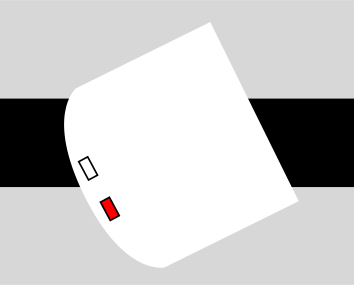
\includegraphics[height=0.35\textwidth]{thymio_half_on_line}}
	\caption{Thymio sur une ligne de ruban adhésif noir}
\end{figure}


Pour suivre une ligne, nous allons utiliser les détecteurs de sol que nous avons déjà utilisé dans le \cref{c.moving}.
Rappelons qu'ils fonctionnent en envoyant de la lumière infrarouge (invisible pour l'oeil humain) et mesurant la quantité de lumière renvoyée.
Si vous poser Thymio sur une de couleur claire, beaucoup de lumière sera réfléchie, et donc l'événement \blksm{lots-of-light} sera déclenché.
Nous avons donc besoin d'une ligne qui déclenchera un événement quand peu de lumière sera réfléchie: \blksm{little-light}.
Ceci est facile à réaliser en imprimant une bande noir, en la peignant ou en utilisant du ruban adhésif noir comme sur la \cref{fig.tape}.
La ligne doit être assez large pour que les deux capteurs de sol la voient quand le robot suit la ligne correctement.
Une largeur de 5 centimètres est suffisante pour que le robot suive la ligne même s'il y a de petites déviations.

Le premier pas pour faire suivre une ligne à Thymio est de le faire avancer s'il est sur la ligne, et que les \emph{deux} capteurs de sol détectent du foncé, et de le faire s'arrêter s'il ne se trouve pas sur la ligne, quand les \emph{deux} capteurs de sol détectent du clair.
Les paires événement-action qui sont illustrées sur \cref{fig.start-stop}.

\trickbox{Assurez-vous d'avoir un câble USB assez long (disons, deux mètres) pour que le robot reste connecté même quand il bouge.
Vous trouverez des rallonges dans les magasins d'informatique.}

\begin{figure}
	\subfigure[Thymio s'arrête, Thymio avance]{ \label{fig.start-stop} \includegraphics[width=0.4\textwidth]{line-forward}}
	\hfill
	\subfigure[Corriger les déviations]{ \label{fig.follow-line} \includegraphics[width=0.4\textwidth]{line-controller}}
	\caption{Un programme pour suivre une ligne}
\end{figure}

\sect{Votre premier contrôleur}

Le prochain pas est de programmer le contrôleur qui suit la ligne :

\begin{itemize}
	\item Si le robot sort de la ligne à \emph{gauche}, comme sur la \cref{fig.one-off}, le capteur \emph{gauche} détectera le sol alors que le capteur \emph{droite} continuera de détecter la ligne ; dans ce cas le robot doit tourner légèrement à \emph{droite}.

	\item Si le robot sort de la ligne à \emph{droite}, le capteur \emph{droite} détectera le sol alors que le capteur \emph{gauche} continuera de détecter la ligne ; dans ce cas le robot doit tourner légèrement à \emph{gauche}.
	
\end{itemize}

Comme nous avons deux conditions, il nous faut deux paires événement-action, comme illustré sur la \cref{fig.follow-line}.

\sect{Régler les paramètres}

Il est assez facile de comprendre que si Thymio dépasse de la ligne à gauche, il doit tourner à droite, comme dans la \cref{fig.one-off}.
La vraie question est plutôt de combien doit-il tourner ?
Si le tour est trop doux, le capteur droit pourrait aussi sortir de la ligne avant que le robot ne tourne assez ; si au contraire le tour est trop aggressif, il pourrait faire sortir le robot de la ligne de l'autre côté.
Dans tous les cas, des tours trop aggressifs peuvent être dangereux pour le robot et ce qu'il transporte.

\importantbox[Paramètres]{
Les \emph{paramètres} sont des valeurs que l'on peut changer sans modifier la structure global des paires événement-action qui forment le programme.}

Dans ce programme, les paramètres que vous pouvez définir sont la vitesse des roues gauche et droite dans chaque bloc d'action moteur.
Vous devrez expérimentr avec ces valeurs jusqu'à ce que le robot bouge de manière \emph{fiable}.
Par fiable, nous entendons que le robot peut réussir à suivre plusieurs fois la ligne.
Comme chaque fois vous placez le robot sur la ligne à différentes positions et pointant dans differentes direction, il faut tester plusieurs fois pour être convaincu que le programme fonctionne.

Thymio doit-il aller vite lorsqu'il est sur la ligne ou, au contraire, lentement ?
En allant vite, vous améliorerez son efficacité pour se déplacer d'un point à un autre mais vous risquez de le faire quitter la ligne avant qu'il ne s'en rende compte, un peu comme si vous allez trop vite en voiture dans un virage serré.
Il faudra donc trouver un bon compromis pour le paramètre vitesse.

Il y a plein de façons différentes de définir les paramètre des blocs d'action moteur qui contrôlent les tours.
Par exemple, une fois que Thymio remarque qu'il quitte la ligne, que doit-il faire ?
S'il fait tourner un moteur dans un sens et l'autre dans le sens oppposé, vous vous assurez qu'il ne quitte pas la ligne mais ses mouvements seront très saccadés.
S'il corrige simplement sa trajectoire en diminuant la vitesse d'une roue, il se déplacera avec fluidité, mais il risque de quitter complètement la ligne.
Là aussi, il faudra trouver un bon compromis.

\exercisebox{\thechapter.1}{
Thymio s'arrête complètement s'il ne détecte plus du tout la ligne.
Modifiez le programme pour qu'il tourne lentement sur lui même vers la gauche jusqu'à ce qu'il retrouve la ligne.
Essayez le sur une igne avec un virage à gauche comme sur la \cref{fig.tape}.
Essayer d'augmenter la vitesse en avant du robot.
Que se passe-t-il lorsque le robot arrive à la fin de la ligne ?
}

\exercisebox{\thechapter.2}{
Modifiez le programme de l'exercice précédent pour que le robot tourne à droite quand il arrive au bout de la ligne.
Que se passe-t-il ?
\vspace{.5em}\\
Il serait bien si on pouvait le \emph{rappeller} quel capteur était le dernier à perdre le contact avec la ligne avec de tourner le robot dans la bonne direction pour retrouver la ligne.
Dans le \cref{ch.states}, nous apprendrons à se rappeller des informations.
}

\exercisebox{\thechapter.3}{
Jouez avec différentes formes de parcours :
\begin{itemize}[noitemsep,nosep,leftmargin=*]
\item Virages doux
\item Virages serrés
\item Zig-zag
\item Ligne plus large
\item Ligne plus étroite
\end{itemize}
Faites la course avec vos amis :
Quel robot suit le plus de lignes différentes avec succès ?
Pour chaque ligne, quel robot la suit dans le moins de temps ?
}

\exercisebox{\thechapter.4}{
Discutez les effets qui les modifications suivantes au Thymio auraient sur les capacités du robot à suivre une ligne :
\begin{itemize}[noitemsep,nosep,leftmargin=*]
\item L'événement des capteurs de sol arrive plus ou moins souvent que 10 fois par seconde ;
\item Les capteurs sont plus éloignés ou proche l'un de l'autre ;
\item Il y a plus que deux capteurs de sol sous le robot.
\end{itemize}
}

% TODO
\chap{Glocken und Pfeifen}
\label{ch.bells}

Lass uns eine Pause von den schwierigen Aufgaben,
wie dem folgen einer Linie machen
und etwas Spass mit dem Roboter haben.
Wir zeigen Dir wie:

\begin{itemize}
\item Komponiere Musik für den Roboter
\item Lass den Roboter auf Musik antworten
\item Lass den Roboter antworten, falls er berührt wird.
\end{itemize}

\sect{Spiele Musik}

Der Thymio-II Roboter enthält ein Synthesizer
und Du kannst diesen programmieren,
um einfache Melodien zu spielen,
indem du den Aktionsblock Musik benutzt \blk{action-music}.

{\raggedleft \hfill Program file \bu{bells.aesl}}

Du wirst kein neuer Beethoven werden
- da nur sechs Noten, in fünf Tonlagen und zwei Tonlängen zur Verfügung stehen -
aber Du kannst eine Melodie komponieren, die dein Roboter einzigartig macht. 
Die Figur Figure~\ref{fig.music} zeigt zwei Ereignis-Aktions Paare,
welche mit einer Melodie antworten,
falls der vordere oder der hintere Schalter berührt wird.
Jedem Ereignis ist eine andere Melodie zugeordnet.

\begin{figure}
\begin{center}
\gr{music}{.4}
\caption{Spiele eine Melodie}
\label{fig.music}
\end{center}
\end{figure}

Die kleinen Kreise sind die sechs Noten.
Die weissen Noten sind lange Tonlängen
und schwarze Noten sind kurze Tonlängen.
Klicke auf den Kreis, um die Tonlänge zu ändern.
Die fünf farbigen, horizontalen Balken stehen für die Tonhöhe.
Klicke auf den \emph{Balken} über oder unter dem Kreis, um den Kreis zu bewegen. 
(Versuche nicht die Kreise zu verschieben (drag and drop), es wird nicht funktionieren). 

\sect{Übung \thechapter.1}

Schreibe ein Programm,
das Dir erlaubt eine Morsebotschaft zu verschicken.
Eine Morsebotschaft wird mit langen und kurzen Tönen kodiert.
(\emph{Striche} für lange Töne und \emph{Punkte} für kurze Töne).
Zum Beispiel wird der Buchstabe \emph{V} mit drei Punkten und einem Strich kodiert.


\sect{Kontrolliere deinen Roboter durch Töne}

Der Thymio-II hat ein Mikrofon.
Das Ereignis \blk{event-clap} findet statt,
wenn ein lautes Geräusch aufgenommen wird, wie z.B. Händeklatschen.
Das Ereignis-Aktions Paar \\ \blk{clap} wird die Bodenlichter einschalten,
wenn du in die Hände klatschst.

\centeredbox{In einer lauten Umgebung kann ein Geräusch eventuell nicht als Ereignis verwendet werden,
da durch den hohen Geräuschepegel dauernd Ereignisse ausgelöst werden.}

\sect{Übung \thechapter.2}

Schreibe ein Programm,
dass den Roboter losfahren lässt,
falls Du in die Hände klatschst und den Roboter stoppt,
falls Du auf den Schalter drückst.

Schreibe ein Programm, das umgekehrt funktioniert:
Der Roboter soll losfahren,
falls Du auf den Schalter drückst und stoppen,
falls Du in die Hände klatschst.

\sect{Gute Arbeit Roboter!}

Haustiere machen nicht immer das,
was wir von ihnen verlangen.
Manchmal brauchen sie einen freundschaftlichen Klaps um sie zu ermutigen.
Genau gleich funktioniert das mit deinem Roboter.
Der Thymio-II enthält ein Berührungssensor, welcher ein Ereignis auslöst \blk{event-tap}, falls dem Roboter kurz auf seine Oberseite geklopft wird. So bewirkt zum Beispiel das Ereignis-Aktions Paar \blk{touch}, dass die Lichter angehen, falls auf die Oberseite des Roboters geklopft wird.

Erstelle ein Programm für dieses Ereignis-Aktions Paar
und das Paar\blk{clap}, welches die Bodenlichter angehen lässt,
falls Du in die Hände klatschst.

{\raggedleft \hfill Program file \bu{whistles.aesl}}

Kannst Du nur die Oberlichter anstellen?
Dies ist schwierig, da ein Klaps immer auch ein Geräusch erzeugt,
welches laut genug sein kann, um ebenfalls die Bodenlichter anzustellen.
Mit ein bisschen Übung wird es Dir jedoch möglich sein,
dem Roboter ein so gefühlsvollen Klaps zu geben,
dass das Geräusch kein Ereignis auslöst.

\sect{Übung \thechapter.3}

Schreibe ein Programm, dass den Roboter vorwärts fahren lässt bis er die Wand berührt. 

\textbf{Warnung} Stell sicher, dass der Roboter langsam fährt und sich dadurch nicht selbst beschädigt.

\chap{A Time to Like}

In Chapter~\ref{ch.pet} we programmed a pet robot who either did or did
not like us. Let us consider a more advanced behavior: a shy pet who
can't make up its mind whether it likes us or dislikes us. Initially,
the pet will turn towards our outreached hand, but then it will turn
away. After a while, it will reconsider and turn back in the direction
of our hand.

{\raggedleft \hfill Program file \bu{shy.aesl}}

The behavior of the robot is as follows. When the right button is
touched the robot turns to the right. When it detects your hand, it
turns to the left but after a while it regrets its decision and turns
back. We know how to construct event-action pairs for the initial turn
\blk{start-turn} and for turning away when your hand is detected
\blk{turn-away}.

The behavior of turning back ``after a while'' can be broken down into
two event-action pairs:

\begin{itemize}

\item \emph{When} the robot starts to turn away $\rightarrow$
\emph{start a timer} for two seconds.

\item \emph{When} the timer runs down to zero $\rightarrow$ \emph{turn}
to the right.

\end{itemize}

We need a new \emph{action} for the first behavior and a new
\emph{event} for the second behavior.

The action is to set an \emph{timer}, which is like an alarm clock
\blk{action-timer}. Normally, we set an alarm clock to an absolute time,
but when I set the alarm clock in my smartphone to an absolute time like
07:00, it tells me the relative time: ``Alarm set for 11 hours, and 23
minutes from now.'' The timer block works the same way: you set the
timer for a certain number of seconds from when the event occurs and the
action happens. The timer can be set for up to four seconds. Click
anywhere within the black circle showing the face of the clock (but not
on the black circle itself). There will be a short animation and then
the amount of time until the alarm will be colored blue.

The event-action pair for the first behavior above is
\blk{turn-clock}.

The timer is set for two seconds. When the event of detecting your
hand occurs, there will be two actions: turning the robot to the left
and setting the timer.

The second behavior needs an event that occurs when the alarm goes off,
that is, when the amount of time set on the timer runs down to zero. The
event block \blk{event-timer} shows a ringing alarm clock.

The event-action pair is \blk{turn-back}, where the robot turns back to
the right when the timer runs down.

\sect{Exercise \thechapter.1}

Write a program that causes the robot to move forward at top speed for
three seconds when the forward button is touched; then it runs
backwards. Add an event-action pair to stop the run by touching the
center button.

\chap{États: Pour ne pas toujours faire la même chose (avancé)}\label{ch.states}

Un programme VPL est composé d'une série de paires événement-action.
Tous les événements sont vérifiés périodiquement et les actions appropriées sont effectuées.
Ceci limite les programmes que nous pouvons créer ; pour aller plus loin nous avons besoin d'une façon de spécifier que certaines paires événement-action sont actives à un certain moment, alors que d'autres ne le sont pas.
Par exemple, dans le \cref{ch.line}, lorsque le robot sort de la ligne, nous aurions aimé qu'il tourne à gauche ou à droite afin de rechercher la ligne dans une direction qui dépend de quel côté il est sorti.

Les états sont disponibles dans le mode \emph{avancé} de VPL.
Cliquez sur \blksm{advanced} avant de travailler sur les projets de ce chapitre.

\sect{Tape, tape}

Dans les programmes que nous avons réalisé jusqu'ici, nous avons souvent \emph{démarré} Thymio en appuyant sur un de ces boutons et \emph{arrêté} Thymio en appuyant sur un autre.
Mais regardez votre ordinateur, normalement, il n'a qu'un seul bouton pour l'allumer ou l'éteindre.
%\blksm{power-button} 
Le bouton se \emph{rappelle} s'il est dans l'état \bu{allumé} ou l'état \bu{éteint}.
Le bouton inclut souvent une petite lumière qui indique son état courrant.

Écrivons un programme qui allume les lumières du robot si vous lui donnez une petite tape et qui les éteigne si vous lui donnez une seconde tape.

{\raggedleft \hfill Programme \bu{tap-allumé-éteint.aesl}}

Il est pratique de décrire ce comportemnet en utilisant un \textit{diagramme d'états} :

\begin{center}
\begin{picture}(240,45)
\thicklines
%\put(0,0){\framebox(240,40){}}
\put(20,20){\circle{40}}
\put(0,0){\makebox(40,40){\textsf{éteint}}}
\put(220,20){\circle{40}}
\put(200,0){\makebox(40,40){\textsf{allumé}}}
\put(40,30){\vector(1,0){160}}
\put(0,30){\makebox(240,10){\textsf{tape $\rightarrow$ allumer}}}
\put(200,10){\vector(-1,0){160}}
\put(0,10){\makebox(240,10){\textsf{tape $\rightarrow$ éteindre}}}
\end{picture}
\end{center}

Ce diagramme comprend deux états indiqués par des cercles, \bu{allumé} et \bu{éteint}.
Depuis l'état \bu{éteint}, le robot peut aller dans l'état \bu{allumé} et revenir, mais seulement en suivant les instructions sur les flèches.
Les instructions décrivent quand une transition d'un état à l'autre peut se produire et quand elle se produit :

\begin{itemize}

\item \textbf{Quand} Thymio est dans l'état \bu{éteint} \textbf{\textit{et}} que l'événement \emph{tape} se produit $\rightarrow$ \emph{allumer} le robot \textbf{\textit{et}} aller dans l'etat \bu{allumé}.

\item \textbf{Quand} Thymio est dans l'état \bu{allumé} \textbf{\textit{et}} que l'événement \emph{tape} se produit $\rightarrow$ \emph{éteindre} le robot \textbf{\textit{et}} aller dans l'etat \bu{éteint}.

\end{itemize}

L'accent mis sur le mot «\,\textbf{\textit{et}}\,» avant la flèche~$\rightarrow$ signifie que deux conditions doivent être remplies pour que la transition se fasse: (a) Le robot doit être dans un certain état et (b) l'événement doit se produire.
Lorsque les deux conditions sont remplies, alors la transition est prise ce qui fait à la fois changer l'état et exécute l'action écrite après la flèche~$\rightarrow$.

Il est important de réaliser que les deux parties de la condition sont indépendantes.
Dans le diagramme ci-dessus (répété ici) :

\begin{center}
\begin{picture}(240,45)
\thicklines
%\put(0,0){\framebox(240,40){}}
\put(20,20){\circle{40}}
\put(0,0){\makebox(40,40){\textsf{éteint}}}
\put(220,20){\circle{40}}
\put(200,0){\makebox(40,40){\textsf{allumé}}}
\put(40,30){\vector(1,0){160}}
\put(0,30){\makebox(240,10){\textsf{tape $\rightarrow$ allumer}}}
\put(200,10){\vector(-1,0){160}}
\put(0,10){\makebox(240,10){\textsf{tape $\rightarrow$ éteindre}}}
\end{picture}
\end{center}

l'événement \emph{tape} apparaît deux fois, mais l'action causée par cet événement \emph{dépend} de l'état dans lequel le robot se trouve.

De façon similaire, dans un même état, différents événements peuvent causer différentes actions et des transitions vers de nouveaux états différents.
Dans le diagramme suivant :

\begin{center}
\begin{picture}(300,80)
\thicklines
%\put(0,0){\framebox(240,80){}}
\put(25,42){\circle{40}}
\put(10,28){\makebox(30,30){\textsf{éteint}}}
\put(280,20){\circle{40}}
\put(265,6){\makebox(30,30){\textsf{allumé2}}}
\put(40,57){\vector(1,0){220}}
\put(280,65){\circle{40}}
\put(265,50){\makebox(30,30){\textsf{allumé1}}}
\put(40,27){\vector(1,0){220}}
\put(0,60){\makebox(295,10){\textsf{bouton gauche $\rightarrow$ s'allumer en vert}}}
\put(0,30){\makebox(295,10){\textsf{bouton droite $\rightarrow$ s'allumer en rouge}}}
\end{picture}
\end{center}

toucher le bouton gauche dans l'état \textbf{éteint} allumer le robot en vert et l'amène dans l'état \textbf{allumé1}, alors que toucher le bouton droite, \emph{dans le même état}, génère une action différente, allumer le robot en rouge, et amène le robot dans un état différent, \textbf{allumé2}.

\sect{Implémenter des diagrammes d'états avec des paires événement-action}

Nous montrons comment \emph{implémenter} le comportement décrit par le diagramme d'état avec des paires événement-action.
Implémenter signifie construire un programme qui fera ce que le diagramme d'états décrit.
La \cref{fig.turn-on-off} montre le programme.
Regardons maintenant les paires événement-action unes à unes.

\begin{figure}
	\subfigure[Une tape pour allumer ou éteindre]{
		\label{fig.turn-on-off1}
		\includegraphics[width=.4\textwidth]{tap-on-off1}
	}
	\hfill
	\subfigure[Une tape pour changer d'état]{
		\label{fig.turn-on-off2}
		\includegraphics[width=.4\textwidth]{tap-on-off2}
	}
	\caption{Une tape qui a des résultats différents en fonction de l'état.}
	\label{fig.turn-on-off}
\end{figure}

Dans la première paire événement-action, l'événement est composé du bloc détection de choc avec une indication d'état \blksm{tap-turn-on-state-only}: \blkc{tap-turn-on}

Un état est indiqué par quatre quartiers d'un cercle, chacun pouvant être soit allumé (orange) ou éteint (blanc).
Dans ce programme, nous utiliserons le quartier en haut à gauche pour indiquer si la lumière du haut du robot est éteinte ou allumée.
Dans cette paire, ce quartier est coloré en blanc, ce qui veut dire que la lumière du robot est éteinte.
Ainsi, cette paire veut dire : si le robot est tapé et que le robot est éteint, allumer le robot.

La seconde paire événement-action veut dire : si le robot est tapé et qu'il est allumé, alors l'éteindre: \blkc{tap-turn-off}
% Ce quartier est coloré en orange, donc le robot est allumé 

Si vous regardez à nouveau le diagramme d'états, vous verrez que seulement la moitié du travail est fait.
En effet, en allumant et éteignant le robot, nous devons aussi changer son état d'\bu{éteint} à \bu{allumé} ou d'\bu{allumé} à \bu{éteint}.
Pour cela nous créons en plus deux paires événement-actions en utilisant le bloc d'action \emph{état} \blksm{action-states}, comme montré sur la \cref{fig.turn-on-off2}.

Le sens de la première paire est : \emph{quand} le robot est tapé \emph{et} que l'état est \emph{éteint}, alors changer l'état à \bu{allumé} : \blkc{tap-state-on}
De même, le sens de la seconde paire est : \emph{quand} le robot est tapé \emph{et} que l'état est \bu{allumé}, alors changer l'état à \bu{éteint} : \blkc{tap-state-off}

La \cref{fig.turn-on-off} montre le programme complet composé de quatre paires ; nous voyons que chaque événement cause à la fois une action sur la lumière et un changement de l'état du robot.
Tant l'action que le changement d'état dépendent de l'état dans lequel le robot se trouve, appellé \emph{état courrant}.

%\newpage

\sect{Dans combien d'états différents Thymio peut-il être?}

L'état est indiqué par un cercle divisé en quatre quartiers.
Quand utilisé avec un événement ou dans le bloc d'action état, chaque quartier peut être :
\begin{itemize}
	\item \textbf{Blanc}: le quartier est \emph{éteint} ;
	\item \textbf{Orange}: le quartier est \emph{allumé} ;
	\item \textbf{Gris}: le quartier n'est pas pris en compte.
\end{itemize}

Par exemple, dans \blksm{states}, les quartiers en haut à gauche et en bas à droite sont allumés, le quartier en haut à droite est éteint, et le quartier en bas à gauche n'est pas pris en compte.
Ceci veut dire que si \blksmpure{states} est associé à un bloc événement, l'événement se produira si l'état est défini soit par :
\begin{center}
\centering \makebox{\raisebox{-1.7em}{\includegraphics[height=4em]{states1}}}\quad ou \quad \makebox{\raisebox{-1.7em}{\includegraphics[height=4em]{states2}}}
\end{center}

Comme chacun des quatre quartiers peut être soit allumé soit éteint, il y a 2 $\times$ 2 $\times$ 2 $\times$ 2 = 16 états possibles :
\begin{quote}
\bu{(éteint, éteint, éteint, éteint)\\(éteint, éteint, éteint, allumé)\\(éteint, éteint, allumé, éteint)\\
\mbox{}\hspace{3em}\ldots\\
(allumé, allumé, allumé, éteint)\\
(allumé, allumé, allumé, allumé)}.
\end{quote}
La \cref{fig.all-states} énumère graphiquement tous ces états.
L'état courant du robot est toujours affiché sur le haut du robot par des arcs de cercles lumineux, par exemple, la \cref{fig.state-leds} montre le robot dans l'état \bu{(allumé, allumé, allumé, allumé)}.

\trickbox[Information]{Lorsqu'un programme démarre, l'état initial est toujours 
\bu{(éteint, éteint, éteint, éteint)}:\quad \blk{state-all-off}}

\trickbox{Si vous n'utiliser pas tous les 16 états possibles, mais par exemple que 2 ou 4, vous êtes libre de décider quel quartier vous utiliser pour représenter votre état.
Aussi, si par exemple vous avez deux choses différentes à encoder dans l'état, et que chacune d'elle a deux valeurs possibles, vous pouvez utiliser deux quartiers indépendemment.
C'est pourquoi la capacité d'\emph{ignorer} un quartier est très utile !
Essayez toujours de rester le plus simple possible.
}

\begin{figure}
	\subfigure[Tous les états possibles de Thymio]{
		\label{fig.all-states}
		
\includegraphics[width = 0.4\textwidth]{all-states}
	} 
	\hfill
	\subfigure[La cercle de LED indique l'état]{
		\label{fig.state-leds}
		\includegraphics[width = 0.4\textwidth]{state-leds}
	}
	\caption{Les états de Thymio et leur représentation}
\end{figure}

\sect{Attraper la souris}

Écrivons un programme qui fasse tourner le robot de droite à gauche à la recherche d'une souris (ou d'un autre objet).
Si le robot détecte une souris avec son capteur avant-gauche, il continue la recherche jusqu'à ce que la souris soit détectée avec son capteur avant-droite.
Puis, il se positionne en face de la souris, comme sur la \cref{fig.cat-mouse}.

{\raggedleft \hfill Programme \bu{mouse.aesl}}

\begin{figure}
	\subfigure[Le chat a trouvé la souris]{\label{fig.cat-mouse}
	\includegraphics[width=0.4\textwidth]{cat-mouse}}
	\hfill
	\subfigure[Recherche avec le capteur avant-droite]{\label{fig.mouse2}
	\includegraphics[width=0.4\textwidth]{mouse2}}
	\caption{Le robot chat cherche la souris}
\end{figure}

La paire événement-action suivante fait tourner le robot à gauche : \blkc{mouse1}
Ceci se produira lorsque le quartier gauche-haut est éteint ; initialement tous les quartiers de l'état sont éteint.

La première paire événement-action dans la \cref{fig.mouse2} attend que la souris soit détectée par le capteur avant-droite.
Notez que le petit carré à côté de ce capteur est blanc pour que l'événement se produise seulement si le capteur le plus à droite seul détecte la souris.
La seconde paire événement-action de la \cref{fig.mouse2} change l'état.

La dernière paire événement-action du programme arrête le robot lorsque la souris est directement en face du capteur avant-centre : \blkc{mouse3}
Pourquoi l'événement de cette paire doit-il dépendre de l'état ?
La raison est que le capteur central détectera aussi la souris durant le scan initial de droite à gauche.
Nous voulons que le robot fasse d'abord un scan complet avant de retourner à la position de la souris ; il est donc nécessaire que cette première détection soit ignorée.
Ceci est accomplit en arrêtant le scan seulement lorsque l'état est \bu{allumé} et ceci arrive que lorsqu'un scan complet a été effectué.

\vfill

\trickbox{
Il vous faudra expérimenter avec la distance de la souris au robot.
Si elle est trop proche du robot, les capteurs à côte du capteur central détecteront aussi la souris, alors que l'événement demande qu'ils ne la détecte \emph{pas}.
}

\vfill

\exercisebox{\thechapter.1}{
Écrivez un programme qui fasse danser le robot : il tourne à gauche sur place durant deux secondes, puis tourne à droite sur place durant trois secondes.
Ces mouvement se répètent indéfiniment.
}

\exercisebox{\thechapter.2 (Difficile)}{
Modifier le programme de suivi de ligne du \cref{ch.line} pour que le robot tourne à gauche quand il sort de la ligne par le côté droite, et qu'il tourne à droite quand il sort de la ligne par le côté gauche.
}
% !TeX root = vpl.tex

\chap{What Next?}\label{ch.next}

This tutorial has introduced the Thymio robot and the Aseba/VPL
environment. The visual programming of the VPL environment is intended
for beginners. To develop more advanced programs for the robot, you will
want to learn how to use the Aseba Studio environment and its AESL
programming language (\cref{fig.studio}).

\begin{figure}[hbt]
\begin{center}
\gr{studio}{.9}
\caption{Aseba Studio environment}\label{fig.studio}
\end{center}
\end{figure}

Programming in Aseba Studio is also based upon the concepts of events
and actions. Since VPL programs are translated into AESL programs,
everything you learned in this tutorial is supported in Studio, but now
you have the flexibility of a full programming language with variables,
expressions, and control statements. Aseba Studio also gives you access
to features of the Thymio that are not available in VPL:

\begin{itemize}
\item You can control all the lights such as the circle of lights
surrounding the buttons.
\item You have more flexibility in synthesizing sound.
\item There is a temperature sensor.
\item A remote control device can be used with the robot.
\end{itemize}

When you are working with Aseba Studio, you can open VPL by clicking on
the button \bu{Launch VPL} in the \emph{Tools} tab at the bottom left of
the window. You can import VPL programs into Aseba Studio simply by
opening its file.

To learn about Aseba Studio and AESL, read the \emph{Programming Thymio} page at:\\
\url{https://aseba.wikidot.com/en:thymioprogram}\\
and follow the link \emph{Text Programming Environment}.

You can find many interesting projects at:\\ \url{https://aseba.wikidot.com/en:thymioexamples}.

The document \textit{From Programming in VPL to
Programming in AESL} explains the translations of the VPL programs in
 this tutorial into AESL:\\
\url{https://aseba.wdfiles.com/local--files/en:thymioprogram/vpl-to-aesl.pdf}.

\vspace{4em}

\informationbox{Have fun and learn a lot!}{Thank you for reading this tutorial!}


\end{document}
